\section{Methodology}\label{sec:methodology}

% \manu{remember our contribution. might be nice to have an intro paragraph that details our process. Here our goal is a rigorous study of various parameters during training. To do so, we place ourselves in a controlled envrionment where we wan modify N settings. Our base model is xxxx.}

% Our goal is to discuss core choices in the visual retriever training process. To do so, we place ourselves in a controlled environment that allows us to ablate parameters of this training. 

Our analysis aims at quantifying the impact of design decisions made when training visual retrievers. In opposition to previous work, we begin our analysis as early as language model modality alignment and iteratively study design choices by modifying design choices independently to reduce confounding factors as much as possible \citep{allenzhu2025physicslanguagemodels1}.


\noindent\textbf{Controlled Experimental Setup.}
A central point of interest is the impact of causal and bidirectional attention masks. While recently studied for textual representation applications \citep{gisserotboukhlef2025pretrainencodersmaskedlanguage, weller2025seqvsseqopen}, we extend the experiment to the vision modality. We use checkpoints released by \citet{gisserotboukhlef2025pretrainencodersmaskedlanguage} which consist in a series of identical 210M parameter transformer models based on the Llama architecture \citep{touvron_llama_2023} trained on 100B tokens that differ only in their attention masking strategy during language model training but that are perfectly identical in terms of training data seen, model size and architecture, learning rate scheduling, etc... The checkpoints we use are \texttt{enc} a bidirectional encoder trained with Masked Language Modeling (MLM), \texttt{dec}, a causal decoder trained with next token prediction, and \texttt{dec-enc} a causal decoder annealed over the end of its textual training by removing the causal mask and switching the training objective to MLM. For the vision tower, we employ the vision component of \texttt{siglip2-base-16b-512} \citep{tschannen2025siglip2multilingualvisionlanguage}, a 86M parameter vision transformer contrastively trained on billions of text-image pairs.
All ablations thus stem from iso-data controlled setups, and as further described, are further trained on the same data sequence, with the same batch sizes, optimizers, schedulers and on the same hardware.
% For this purpose, we leverage the checkpoints released by , which provide this rigorously controlled setting. In addition, we include a decoder model from this work that was annealed with MLM objectives, allowing us to evaluate whether decoders can effectively transition into encoders prior to modalities alignment~\citep{gisserotboukhlef2025pretrainencodersmaskedlanguage,weller2025seqvsseqopen}. 
%We use SigLIP2-16B-512 as vision encoder.
% \paul{ablation runs table?}
%The full set of ablation model configurations is summarized in Appendix~\ref{appendix:ablation_models}.

\begin{figure}[t]
    \centering
    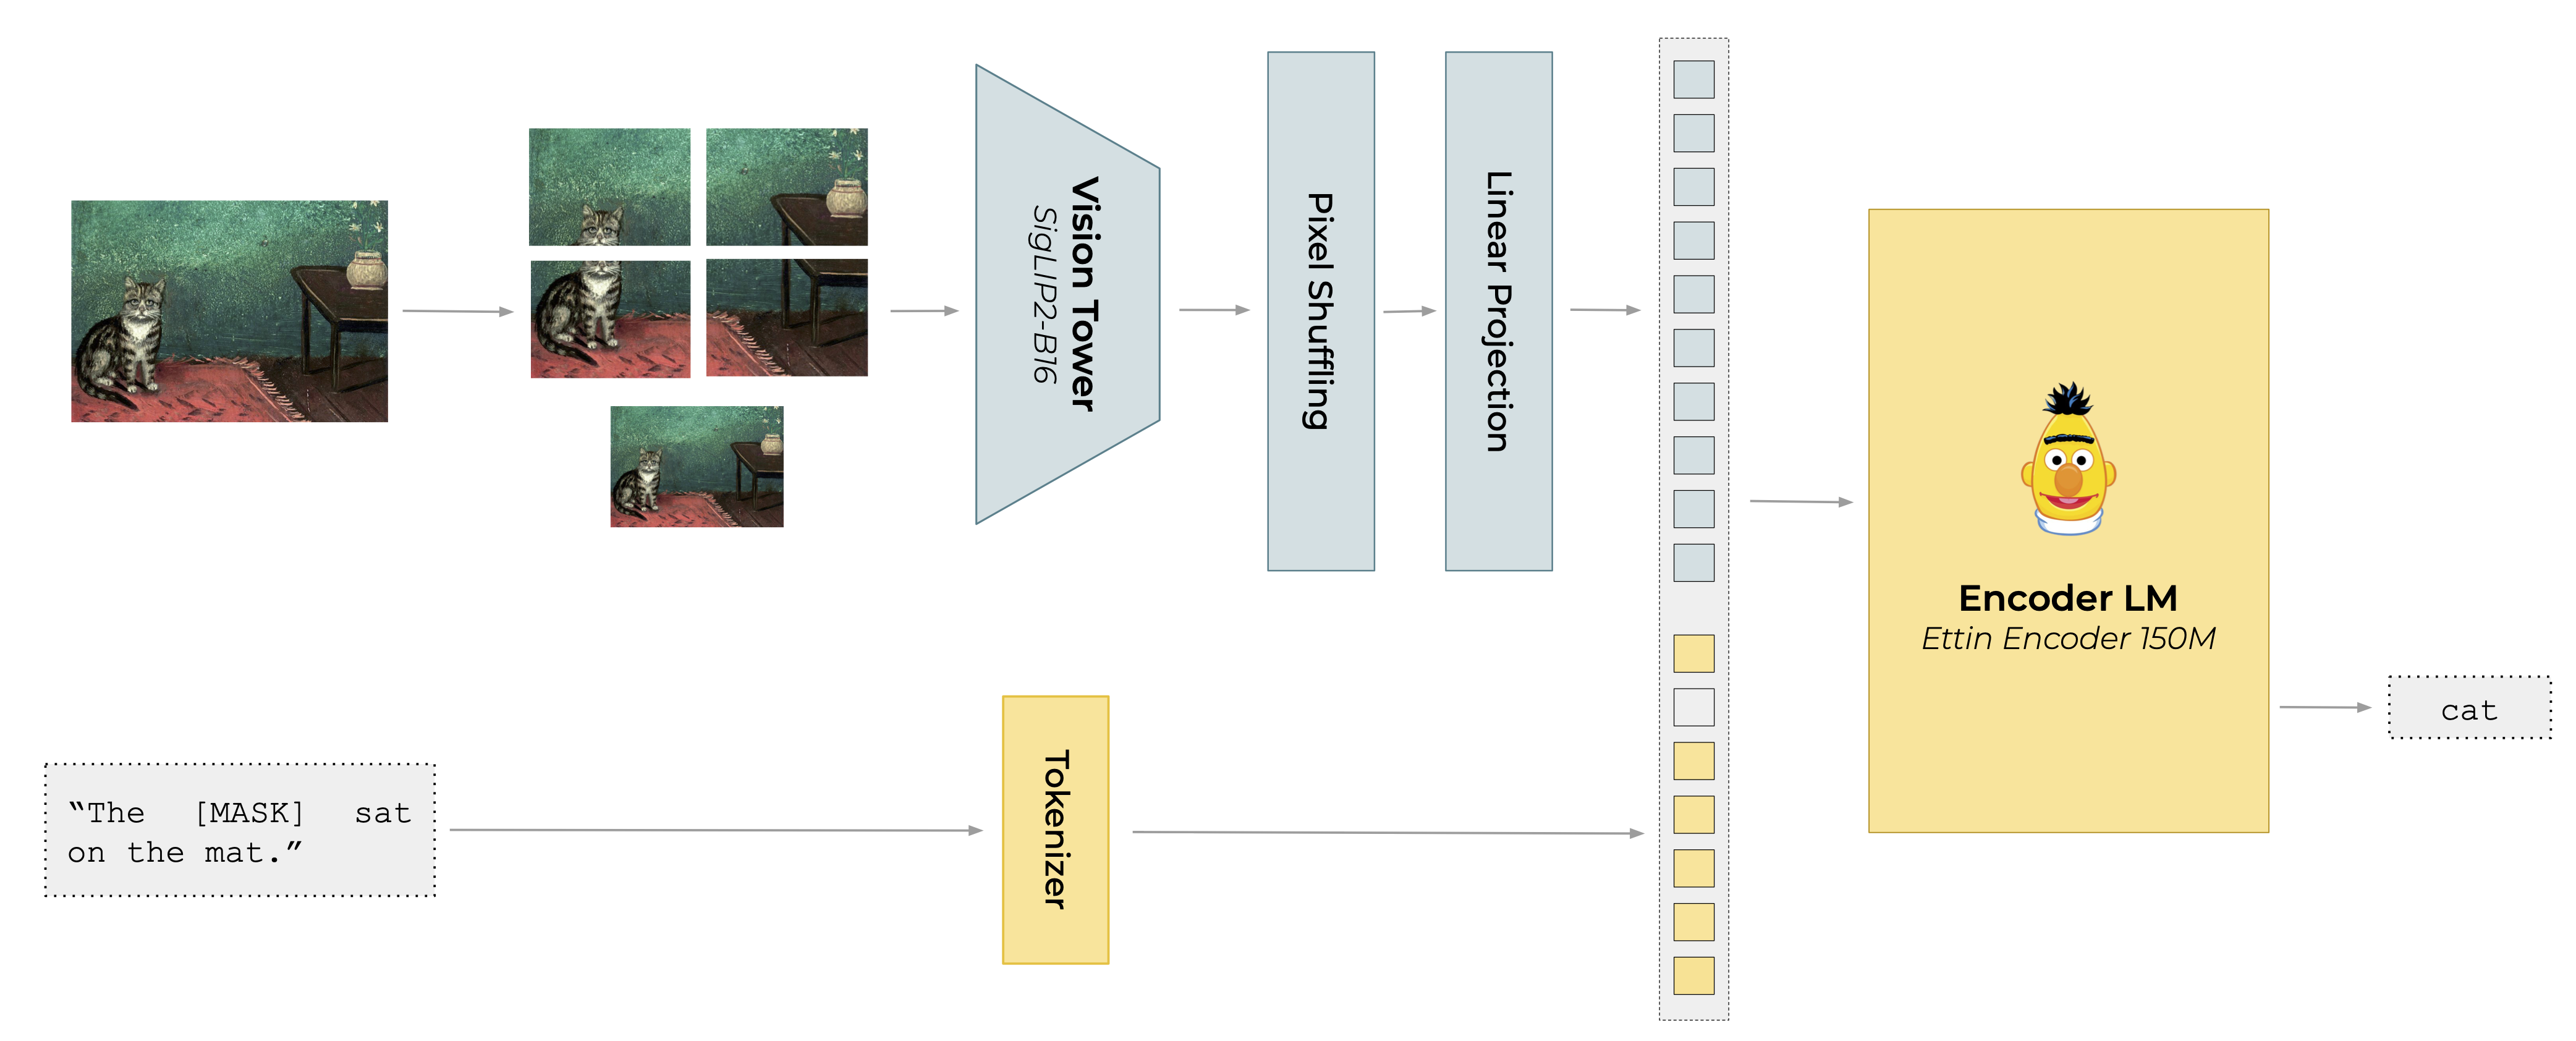
\includegraphics[width=0.99\textwidth]{figures/vbert_architecture.png}
    \caption{
    \textbf{MLM-based early fusion architecture.} The visual encoder produces patch representations, which are passed to a language model. 
    %We apply pixel shuffling to compress the visual representations produced by the vision tower.
    Our end-to-end bidirectional attention fused architecture is trained with Masked Language Modeling objectives and is perfectly suited for sequence and token-level representation tasks.}
    \label{fig:lf_architecture}
\end{figure}

\noindent\textbf{Model Architecture.}  
Our analysis are not centered around model architectures and to draw broadly applicable insights, we design vision-language models following current standard training practices.  In line with most recent work, we employ the early fusion architecture \citep{alayrac2022flamingovisuallanguagemodel} illustrated in Figure~\ref{fig:lf_architecture}, in which visual patch embeddings produced by the vision encoder are projected into the language model input embedding space and concatenated with text token embeddings to encourage joint processing ~\citep{li2022blipbootstrappinglanguageimagepretraining,alayrac2022flamingovisuallanguagemodel,wang2024qwen2vlenhancingvisionlanguagemodels,yang2025qwen251mtechnicalreport,marafioti2025smolvlmredefiningsmallefficient}. As described in \autoref{sec:modality-align}, we generalize the training loss to function both with causal and masked language modeling objectives.  
To handle dynamic resolutions, we split large images into 512$\times$512 pixel tiles as expected by the SigLIP encoder\textcolor{red}{\footnote{\textcolor{red}{Images are downscaled (or upscaled) so that the lengths and widths reach a multiple of 512 pixels to preserve the aspect ratio, padding is used on the smaller side when necessary (i.e. a 1024x1000 px image would be padded to 1024x1024 px).}}}. Following current standard practices, we further process a downscaled version of the full image to improve inter-tile consistency and global visual understanding~\citep{lin2023sphinxjointmixingweights,ye2023ureaderuniversalocrfreevisuallysituated}. \textcolor{red}{The vision tower produces 1024 pixel patch representations for each tile\footnote{\textcolor{red}{The SigLIP tower takes 512x512 px images and process them by 16x16 px patches \citep{dosovitskiy_image_2020}. This results in $(512/16)^2=1024$ patches.}}, which we  compress to 64 tokens through \textit{pixel shuffling}~\citep{shi2016realtimesingleimagevideo}} with a compression ratio $r=4$, following prior work on models of comparable size~\citep{marafioti2025smolvlmredefiningsmallefficient}. \textcolor{red}{We highlight the impact of image resolution and this parameter on the number of visual tokens in Appendix~\ref{appendix:visual_tokens}}.

% To handle dynamic resolutions, we split large images into 512$\times$512 pixel patches as expected by the SigLIP encoder, and further concatenate a downscaled version of the full image to improve inter-patch consistency and global visual understanding following current standard practices ~\citep{lin2023sphinxjointmixingweights,ye2023ureaderuniversalocrfreevisuallysituated}. To compress the information from sequences of large images, we apply pixel shuffling~\citep{shi2016realtimesingleimagevideo} with a ratio of $r=4$, following prior work on models of comparable size~\citep{marafioti2025smolvlmredefiningsmallefficient}.

% Note that we do not employ vision encoders with native resolution and RoPE-2D, as our focus is solely on single image representation learning using compact models. In this context, the additional computational overhead of such encoders is not justified.\paul{draft, I have to read qwen2vl carefully and understand the tradeoff more clearly}



% \noindent\textbf{Controlled Experimental Setup.}  
% We build on the publicly available checkpoints of \citet{gisserotboukhlef2025pretrainencodersmaskedlanguage}, which provide a fully controlled environment: all models share identical architectures, parameter counts, training datasets, and schedules, and differ only in the use of causal versus bidirectional attention masks. In addition, we include a decoder model from this work that has been annealed with MLM objectives, allowing us to evaluate whether decoders can effectively transition into encoder-like behavior. The full set of ablation models configurations is summarized in Table~\ref{tab:ablation_models}.

\noindent\textbf{Training Procedure.} Our experiments focus on retrieval performance. We employ a standard biphasic training procedure, in which we first run modality alignment to train a pretrained textual language model to understand visual inputs through language modeling objectives  ~\citep{liu2023visualinstructiontuning} (\autoref{sec:modality-align}), then rely on a second text-image contrastive learning phase to learn efficient image representations ~\citep{radford2021learningtransferablevisualmodels} (\autoref{sec:contrastive_posttraining}). We further describe the general setup, and detail specific modifications to the default training procedure in the experiment section.

\subsection{Modality Alignment}
\label{sec:modality-align}
We align the vision encoder tower with the language model by training the image embedding projection layer to map visual features into the language model embedding space. The pretrained language model is also fine-tuned with Low-Rank Adapters (LoRA) \citep{hu2021loralowrankadaptationlarge}, allowing both image and text models to adapt jointly while reducing the risk of monomodal performance collapse \citep{alayrac2022flamingovisuallanguagemodel,liu2023visualinstructiontuning,laurençon2024mattersbuildingvisionlanguagemodels,mckinzie2024mm1methodsanalysis,marafioti2025smolvlmredefiningsmallefficient}.

\noindent\textbf{Alignment Loss.} 
For decoder‑based models, we train with Causal Language Modeling (CLM) loss on the text tokens, as standardly done in VLM modality alignment:
\begin{equation}
\mathcal{L}_{\text{CLM}}
  = -\sum_{t=1}^{T} \log P_{\theta}\!\bigl(x_t \mid x_{<t}\bigr),
\end{equation}

where $x_{<t}$ denotes all tokens preceding position $t$. We generalize this training scheme to bidirectional encoders models, by using the Masked Language Modeling (MLM) loss on the textual tokens:
\begin{equation}
\mathcal{L}_{\text{MLM}}
  = -\sum_{t \in \mathcal{M}} \log P_{\theta}\!\bigl(x_t \mid x_{\backslash\mathcal{M}}\bigr),
\end{equation}
where $\mathcal{M}$ is the set of masked token positions and
$x_{\backslash\mathcal{M}}$ is the input with those tokens masked out.


\noindent\textbf{Modality Alignment Corpus.} Models are modality aligned on a large corpus in large parts derived from The Cauldron 2~\citep{laurençon2024mattersbuildingvisionlanguagemodels} and Docmatix~\citep{laurençon2024building}. Our objective being to train document focused retrieval models, we use an adjusted training mixture that upsamples images containing text and documents with varying level of complexities. Our final training corpus consists of approximately 2B text tokens, and includes diverse sources such as web pages, books, and scientific papers. Mixture details are given in Appendix~\ref{appendix:alignment_mixture}. We note that controlling the exact data distribution during this phase enables the models we train to specialize early and achieve good document focused downstream performances which many large models struggle with \citep{liu_improved_2023}.

\noindent\textbf{Parameters.} All models are trained using a masking ratio of 0.5 and user-prompt masking to avoid overfitting on chat-template format~\citep{huertaenochian2024instructionfinetuningdoesprompt,shi2024instructiontuninglossinstructions,allal2025smollm2smolgoesbig}. We employ WSD scheduler~\citep{hu2024minicpmunveilingpotentialsmall} with the first 5\% of the training as warmup, the last 20\% as decay and a maximum learning rate of 1e-4. The ablation models are aligned on 3.5B tokens. We provide additional details on the training setup in Appendix~\ref{appendix:implementation_details}.

\subsection{Contrastive Post-Training}
\label{sec:contrastive_posttraining}
Once the language model has learned to process image tokens jointly with text tokens, we specialize models through a contrastive post-training stage designed to enhance the semantic representation of the output embeddings produced by the model \citep{reimers_sentence-bert_2019}. 

% We use a contrastive learning objective to modify the latent space of our base model to adapt it for similarity tasks. 

%We generate embeddings by mean pooling \maxou{cite paper backing this choice} token embeddings for encoder-based models, and by selecting the EOS token embeddings for decoder-based models \maxou{potentially here too? e.g. Qwen3-Embeddings}. 

\noindent\textbf{Post-training Pairs.} The post-training dataset used as starting point in our ablations comprises 118\textcolor{red}{k} document-query pairs from the ColPali corpus~\cite{faysse2025colpaliefficientdocumentretrieval} as well as another 118\textcolor{red}{k} of natural image-description pairs from the MSCOCO train set~\citep{lin2015microsoftcococommonobjects}.

\textbf{Contrastive Loss.} We employ the InfoNCE loss~\citep{oord2019representationlearningcontrastivepredictive}, defined as

\begin{equation}
\mathcal{L}_{\text{InfoNCE}}(\mathbf{q},\mathbf{d^+})
  =-\log\frac{\Phi(\mathbf{q},\mathbf{d^+})}{\Phi(\mathbf{q},\mathbf{d^+}) + \sum_{\mathbf{d^-}\in\mathcal{N}_q}\Phi(\mathbf{q},\mathbf{d^-})},
\end{equation}

where $\mathbf{d^+}$ denotes the positive target for the query $\mathbf{q}$, $\mathcal{N}_\mathbf{q}=\mathcal{N}_\mathbf{q}^{\text{in}} \cup \mathcal{N}_\mathbf{q}^{\text{hard}}$ the set of negative targets (in-batch and hard negatives when mentioned), and $\Phi(\mathbf{q},\mathbf{d})$ a similarity function between the token(s) of the query and the documents.\footnote{We use the last (EOS) token for causal models, and mean pool all sequence tokens for bidirectional encoders for single-vector models. Alternatively, we use all document and query tokens without pooling for late interaction matching \citep{faysse2025colpaliefficientdocumentretrieval}. Details in Appendix~\ref{appendix:similarity_functions}}. 
For general-domain post-training we compute the loss symmetrically~\citep{radford2021learningtransferablevisualmodels}.

\textbf{Batches Curation.} In contrastive learning, batch diversity critically impacts retrieval entropy. Overly heterogeneous batches lead to trivial retrievals, while curated batches yield richer training signals. We employ task-aware batching~\citep{li2023generaltextembeddingsmultistage}, grouping documents by source to ensure a homogeneous batch composition.


\subsection{Ablation Evaluation Setup}


The contrastively trained models are evaluated on retrieval and zero-shot classification tasks across multiple domains. Although the main focus remains document retrieval capabilities, evaluated by aggregating scores from the ViDoRe and ViDoRe v2\footnote{\label{fn:vidorev2}We report only the English splits of ViDoRe v2, as our base models are trained on English data only.} \citep{macé2025vidorebenchmarkv2raising} benchmarks (nDCG@5), we also assess more generalist image retrieval capabilities by selecting tasks from MIEB~\citep{xiao2025miebmassiveimageembedding}. For natural image retrieval, we aggregate MSCOCO retrieval ~\citep{lin2015microsoftcococommonobjects} and Flickr30k retrieval (nDCG@10) \citep{plummer2016flickr30kentitiescollectingregiontophrase} test sets. Finally, following practices in \citep{muennighoff_mteb_2022}, we assess both zero-shot and fine-tuning abilities of our models on general classification tasks. Specifically, we measure classification accuracy by fine-tuning a logistic regression head on top of our model's embedding on Stanford Cars~\citep{6755945} and Food101~\citep{10.1007/978-3-319-10599-4_29}, and we evaluate zero-shot performance on FER2013~\citep{khaireddin2021facialemotionrecognitionstate} and EuroSAT~\citep{helber2019eurosatnoveldatasetdeep} and aggregate the results.

